\documentclass[11pt,aspectratio=1610]{beamer}
\usepackage{fbb}
\usetheme{CambridgeUS}
\beamertemplatenavigationsymbolsempty
\usepackage[utf8]{inputenc}
\usepackage{amsmath,adjustbox,mathtools}
\usepackage{amsfonts}
\usepackage{hyperref}
\usepackage{graphicx}
\usepackage{xpatch}
\usepackage{makecell}
\usepackage{tabularx}
\usepackage{csquotes}
\usepackage{adjustbox}
\setbeamertemplate{caption}{\raggedright\insertcaption\par}
\usepackage{minted}
\usetheme{default}
\usecolortheme{default}


% Définition des couleurs
\definecolor{schTag}{RGB}{204, 0, 0}       % Rouge pour les balises
\definecolor{schAttr}{RGB}{0, 0, 153}      % Bleu pour les attributs
\definecolor{schValue}{RGB}{0, 102, 0}     % Vert pour les valeurs
\definecolor{schBg}{RGB}{245, 245, 245}    % Fond gris clair

% Configuration de minted
\setminted{
  bgcolor=schBg,
  frame=single,
  framesep=2mm,
  linenos=true,
  breaklines=true,
  fontsize=\small,
}


\usepackage{pgfplots}
\usepackage{tikz}
\usetikzlibrary{shapes,calc,matrix,decorations.markings,decorations.pathreplacing,positioning, intersections,backgrounds,through,hobby}
\usepackage[english]{babel}
%\AtBeginSection[]
%{\begin{frame}
% \frametitle{}  
%\setlength{\itemsep}{.5cm}
% \tableofcontents[currentsection,
%                  hideothersections,
%		  sectionstyle=hide/hide/hide,
%                  subsectionstyle=show/show/show/hide
%                   ]
% \end{frame} 
% }

%\AtBeginsection[]
%{\begin{frame}
% \frametitle{}  
% \tableofcontents[currentsection,
%	 	  currentsection,
%		  sectionstyle=show/hide,
%                  sectionstyle=show/shaded/hide
%                   ]
% \end{frame} 
% }


\AtBeginSection[]
{
  \begin{frame}
    \tableofcontents[
      currentsection,       % Met en évidence la section courante
      sectionstyle=show/shaded, % Sections : courante en évidence, autres en grisé
      subsectionstyle=hide  % Cache toutes les sous-sections
    ]
  \end{frame}
}
 
 

\AtBeginSubsection[]
{
  \begin{frame}
    \tableofcontents[
     currentsection, % Affiche uniquement la section courante
      hideothersubsections, % Cache les sous-sections des autres sections
      sectionstyle=show/hide, % Cache les autres sections
      subsectionstyle=show/shaded/hide % Sous-section courante en évidence, les autres en grisé
    ]
  \end{frame}
}


\setbeamertemplate{sections/subsections in toc}[square]
\setbeamertemplate{bibliography item}[sqare]
\setbeamertemplate{itemize item}[square]
\setbeamertemplate{enumerate item}[square]
\setbeamertemplate{itemize subitem}[square]




\setbeamertemplate{sections/sections in toc}[square]
\setbeamertemplate{itemize item}[square]
\setbeamertemplate{enumerate item}[square]
\setbeamertemplate{itemize subitem}[square]

\usepackage[style=verbose,citestyle=authoryear,isbn=true,url=false,
doi=true,backend=biber,maxbibnames=9, maxcitenames=4]{biblatex}
\addbibresource{/home/mgl/Bureau/Travail/Communications_et_articles/bibliographie_commune/biblio.bib}
\renewcommand*{\bibfont}{\tiny} 

\usepackage{tikz}
\usetikzlibrary{shapes,calc,matrix,decorations.markings,decorations.pathreplacing,positioning, intersections,backgrounds}
\tikzstyle{bag} = [align=center]

\date[24 mars 2026]{24 mars 2026}
\author[Matthias \textsc{Gille Levenson}]{\\~\\ Matthias \textsc{Gille Levenson}\\   {\scriptsize Université Versailles Saint Quentin (UVSQ) \& École Normale Supérieure de Lyon, France}\\ {\tiny matthias [dot] gille [-] levenson [at] ens-lyon [dot] fr}\vspace{-1cm}}
\title[Les schémas]{Session 3: Les schémas\\ {\small Atelier Humanités Numériques \\ Lyon}}
%\titlegraphic{\hspace{0.5cm}\includegraphics[scale=0.21]{/home/mgl/Bureau/Travail/admin/logos/ensl.png}\hspace{0.5cm}\includegraphics[scale=0.23]{/home/mgl/Bureau/Travail/admin/logos/ciham.pdf}\hspace{0.5cm}}
\usepackage[justification=centering]{caption}
\begin{document}
\maketitle

\section{Introduction}


\section{Les schémas}
\subsection{Avantages de l'utilisation des schémas}
\begin{frame}{À quoi sert un schéma ?}
\begin{itemize}
\item Un schéma vérifie si les données sont correctement formatées.
\item Un schéma définit des règles concernant ce qui est autorisé et ce qui ne l'est pas dans une structure de données XML
\item Appliqué à un codage de texte, un schéma est un modèle du \enquote{texte}, c'est-à-dire une \textbf{représentation formelle} du texte.
\item D'un point de vue pratique, cela permet d'harmoniser votre encodage et constitue une \textbf{étape importante vers l'interopérabilité}
\end{itemize}
\end{frame}


\begin{frame}{Intégration du schéma dans vos sessions d'encodage}
Certains éditeurs XML utilisent le schéma comme outil pour faciliter le codage : 
\begin{figure}
 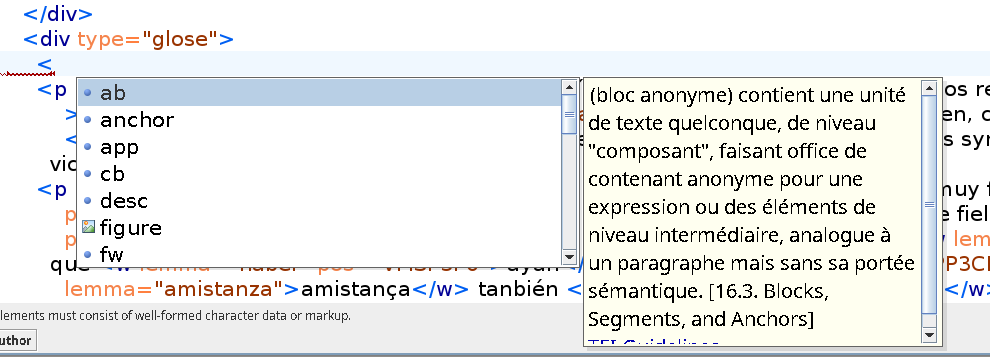
\includegraphics[height=.5\textheight]{img/example_tei.png}
 \caption{L'éditeur XML Oxygen vous permet de choisir parmi les éléments autorisés}
\end{figure}
\end{frame}

\begin{frame}{Les schémas}
\begin{itemize}
\item Un schéma est un document qui sert à contrôler la qualité d'un encodage.
\item La TEI fournit des \textbf{règles} (les \textit{Guidelines}, lisibles par l'homme) et leur \textbf{formalisation} (\textit{schémas}, lisibles par machine) afin de vérifier la validité d'un document donné
\item D'un point de vue abstrait, le schéma représente la formalisation de \textit{votre} modélisation d'un texte ou d'un genre donné.
\end{itemize}
\end{frame}


\begin{frame}{Les schémas}
\begin{center}
\begin{figure}
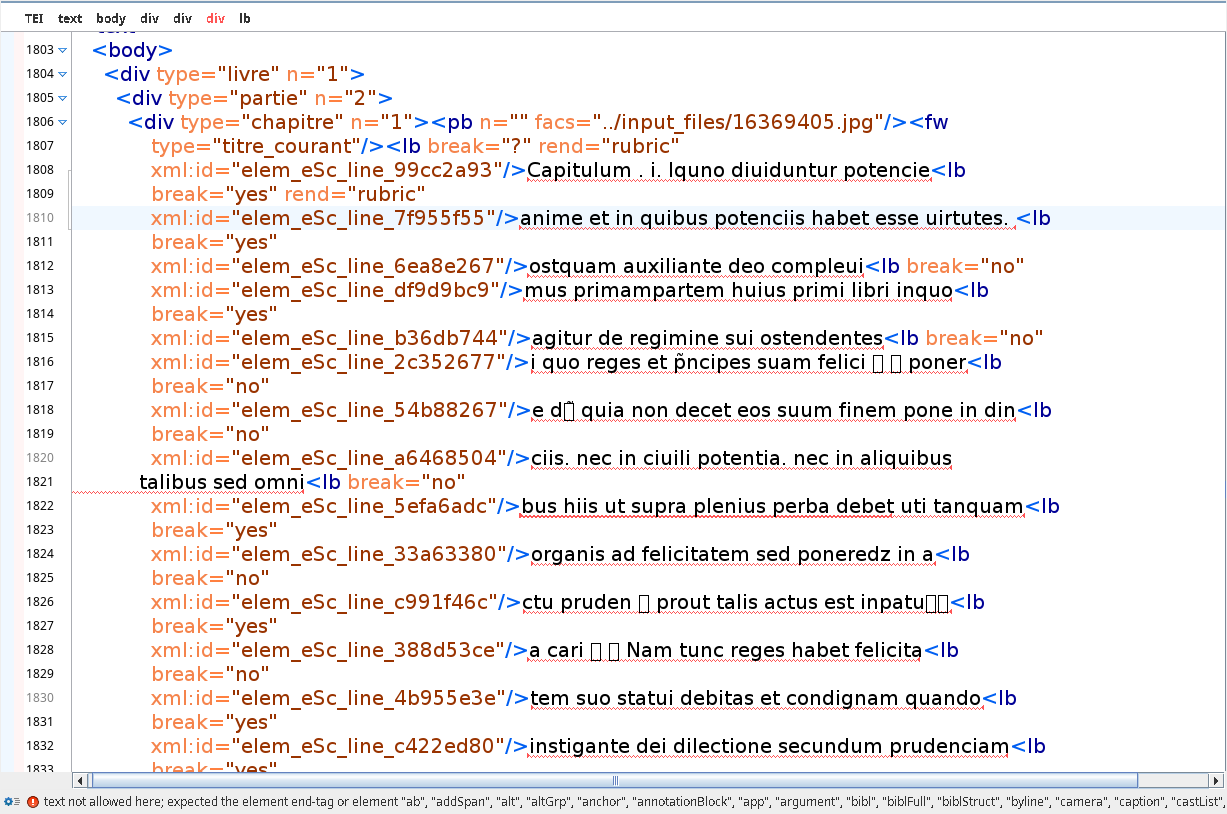
\includegraphics[height=.75\textheight]{img/validation.png}
\caption{Ce fragment est \textit{bien formé}, mais il n'est pas \textit{valide} selon le schéma XML-TEI. Ces lignes devraient être encadrées par un paragraphe \texttt{p} ou un bloc anonyme \texttt{ab}.}
\end{figure}
\end{center}
\end{frame}


\begin{frame}{Formats de schémas}

Il existe plusieurs formats de schéma. Les plus importants sont les suivants :
\begin{itemize}

\item Définition de type de document (DTD)
\item Schéma XML (format XSD)
\item Schémas Relax NG (RNG) et leur version compacte (RNC)
\end{itemize}
\end{frame}


\subsection{Les schémas et la TEI I}
\begin{frame}{Les TEI subsets}
\begin{center}
\begin{figure}
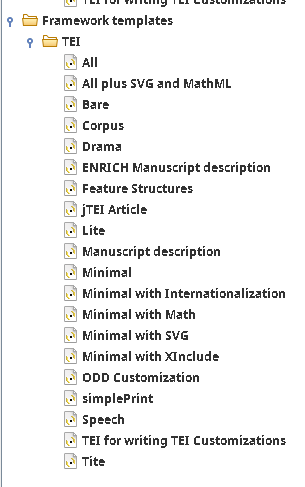
\includegraphics[height=.6\textheight]{img/schemas.png}
\end{figure}
\begin{itemize}
\item Il existe plusieurs schémas TEI.
\item En tant que norme scientifique, le TEI doit être adapté aux besoins de l'utilisateur.ice
\end{itemize}
\end{center}
\end{frame}


\begin{frame}{Pourquoi devriez-vous créer votre propre personnalisation TEI ?}
\begin{center}
\begin{itemize}
\item Considérez la TEI comme un outil permettant de modéliser votre objet textuel
\item Vous n'aurez probablement pas besoin de tous les outils conceptuels fournis par le Consortium TEI.
\item Si vous êtes médiéviste, vous souhaiterez peut-être écarter les éléments appartenant à la section \enquote{Transcriptions du discours} de la TEI (hélas !)
\item Votre schéma sera la formalisation de votre façon de voir le texte, et vous devez le rendre aussi précis que possible.
\end{itemize}
\end{center}
\end{frame}


\begin{frame}{Deux méthodes principales}
\begin{center}
\begin{itemize}

\item La méthode par inclusion : partez de zéro, ajoutez les éléments dont vous avez besoin

\item La méthode par exclusion : partez d'un schéma prédéfini, supprimez les éléments dont vous n'avez pas besoin

\pause\item  Je vous recommanderais d'adopter la première approche...

\pause\item ou du moins de partir d'une spécification prédéfinie qui répond à certains de vos besoins (nous verrons cela plus tard).

\pause\item Il est essentiel de maîtriser les lignes directrices pour savoir ce qui est possible pour votre projet.

\end{itemize}
\end{center}

\end{frame}



\begin{frame}{Ne réinventez pas la roue !}
\begin{center}
\begin{figure}
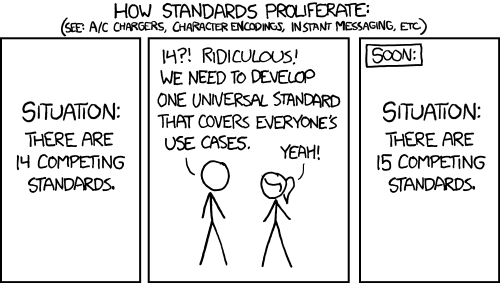
\includegraphics[width=.4\textwidth]{img/standards.png}
\caption{\url{https://xkcd.com/927/}}
\end{figure}
\begin{itemize}
\item Vous devez définir et adapter les règles TEI à votre propre projet

\item Cependant, les problèmes de modélisation auxquels vous serez confronté ne sont probablement \textit{pas} nouveaux

\item Ne réinventez pas la roue ! 

\item Recherchez ce qui a déjà été fait pour des problèmes similaires et essayez les solutions proposées !

\item Et (pour commencer), évitez d'inventer ou de créer de nouveaux éléments.
\end{itemize}
\end{center}
\end{frame}


\subsection{Les schémas and la TEI II: l'ODD}
\begin{frame}{Is that all, folks ?}
\begin{center}
\begin{itemize}
\item Créer un schéma spécifique est un bon début.

\pause\item Que manque-t-il alors ? \pause \textit{De la documentation}.

\pause\item Vous souhaitez maintenant expliquer vos règles à votre supérieur, à vos collègues et à vos enfants. Vous devez rédiger cela \textit{en langage naturel}.

\pause\item Quoi de mieux qu'un document TEI pour décrire un autre document TEI ?
\end{itemize}
\end{center}
\end{frame}








\begin{frame}{Here comes the ODD}
\begin{itemize}
\item ODD signifie \enquote{One Document Does it All}

\item Un ODD est un document TEI qui sert à créer à la fois la documentation et le schéma dans un seul et même document.

\item Lecture recommandée : \fullcite{burnard_WhatTEIConformance_2019}
\end{itemize}
\end{frame}


\begin{frame}{Un Document pour les Contrôler Tous}
Un ODD contient :

\begin{itemize}

\item les éléments lisibles par machine utilisés pour \textit{valider} une édition

\item les éléments lisibles par l'homme utilisés pour \textit{documenter} celle-ci

\end{itemize}
\end{frame}






%\begin{frame}{Basic TEI schema concepts \parencite{vigliantiOneDocumentDoesitall2019a}}
%\begin{itemize}
%\item \textbf{Module}
%\item \textbf{Model class} (or element class)
%\item Attribute class
%\item Element
%\item Classes
%\item datatypes
%\item macros
%\end{itemize}
%You will manipulate the items in bold for a start. 
%\end{frame}


\begin{frame}
       \begin{columns}
          \column{0.55\linewidth}
\begin{figure}
             \centering
 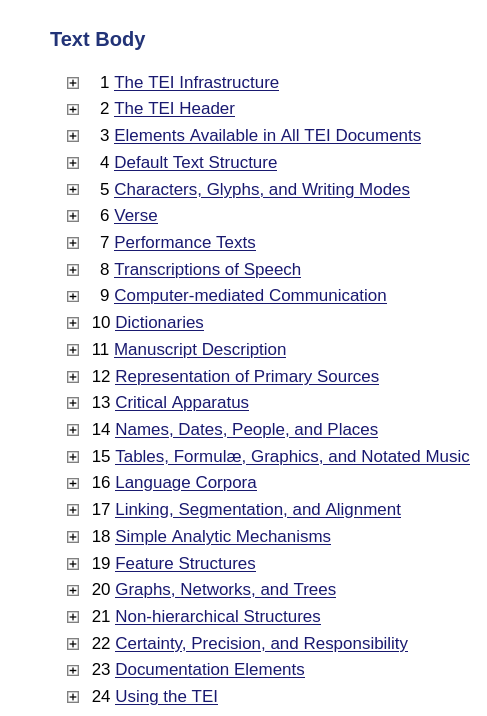
\includegraphics[width=.6\textwidth]{img/tei_modules.png}
\end{figure}
           \column{0.40\linewidth}
\begin{itemize}
\item Le TEI est organisé en modules \textit{thématiques} qui correspondent aux chapitres indiqués plus haut
\item Le module est la formalisation informatique du chapitre.
\end{itemize}
         \end{columns} 
    \end{frame}


\begin{frame}{TEI as modules}
\begin{itemize}
\item 22 modules

\item Chaque module est associé à une liste d'éléments. Si vous désactivez un module, ces éléments ne seront plus accessibles. 

\item 4 modules principaux : \texttt{tei}, \texttt{core}, \texttt{header} et \texttt{textstructure}, pratiquement obligatoires

\end{itemize}
\end{frame}



\begin{frame}{Un \textsc{ODD} n'est PAS un schéma}

\begin{itemize}
\item Il s'agit d'un \textbf{document TEI} utilisé pour générer des schémas.

\item Il doit être \textbf{converti} en schéma (et en documentation, le cas échéant).

\item Le schéma obtenu (généralement au format RNG) est le document que vous utiliserez pour valider vos documents XML.

\item N'essayez pas de valider vos fichiers par rapport aux ODD !
\end{itemize}
\end{frame}





\subsection{ROMA}
\begin{frame}{Création de fichiers ODD et de schémas avec ROMA}

% Image vers ROMA
\begin{itemize}
\item ROMA, géré par Raffaele Viglianti (responsable), Peter Stadler et Bryan Wang.

\item ROMA est une interface simple permettant de concevoir des ODD et de créer des schémas

\item URL : \url{https://roma.tei-c.org/}
\end{itemize}
\end{frame}


\begin{frame}{A quick look at our ODD}
With ROMA, you can easily design your own ODD:
\begin{itemize}
\item Inclure ou exclure des modules spécifiques

\item Supprimer complètement des éléments (ils ne seront plus autorisés)

%\item Supprimer partiellement des éléments (ils ne seront autorisés que dans des contextes spécifiques)

\item Imposer des contraintes sur les types d'attributs ou les valeurs d'attributs

\item Rendre certains attributs obligatoires

\item etc.
\end{itemize}
\end{frame}


\begin{frame}{Création de fichiers ODD et de schémas avec ROMA}

% Image vers ROMA
\begin{itemize}
\item Je m'intéresse au codage d'un manuscrit médiéval. Comment puis-je créer le fichier ODD le plus adapté avec ROMA ?

\item Je souhaite m'assurer que l'utilisateur utilise l'attribut \texttt{@n} pour chaque élément de début de page (\texttt{pb}). Comment puis-je procéder ?

\item Je souhaite supprimer les éléments \texttt{div1}, \texttt{div2}, ..., \texttt{div7}, afin que les divisions soient balisées uniquement avec des éléments \texttt{div} typés et identifiés. 
\end{itemize}
\end{frame}

\begin{frame}{Création de fichiers ODD et de schémas avec ROMA}
\begin{figure}
 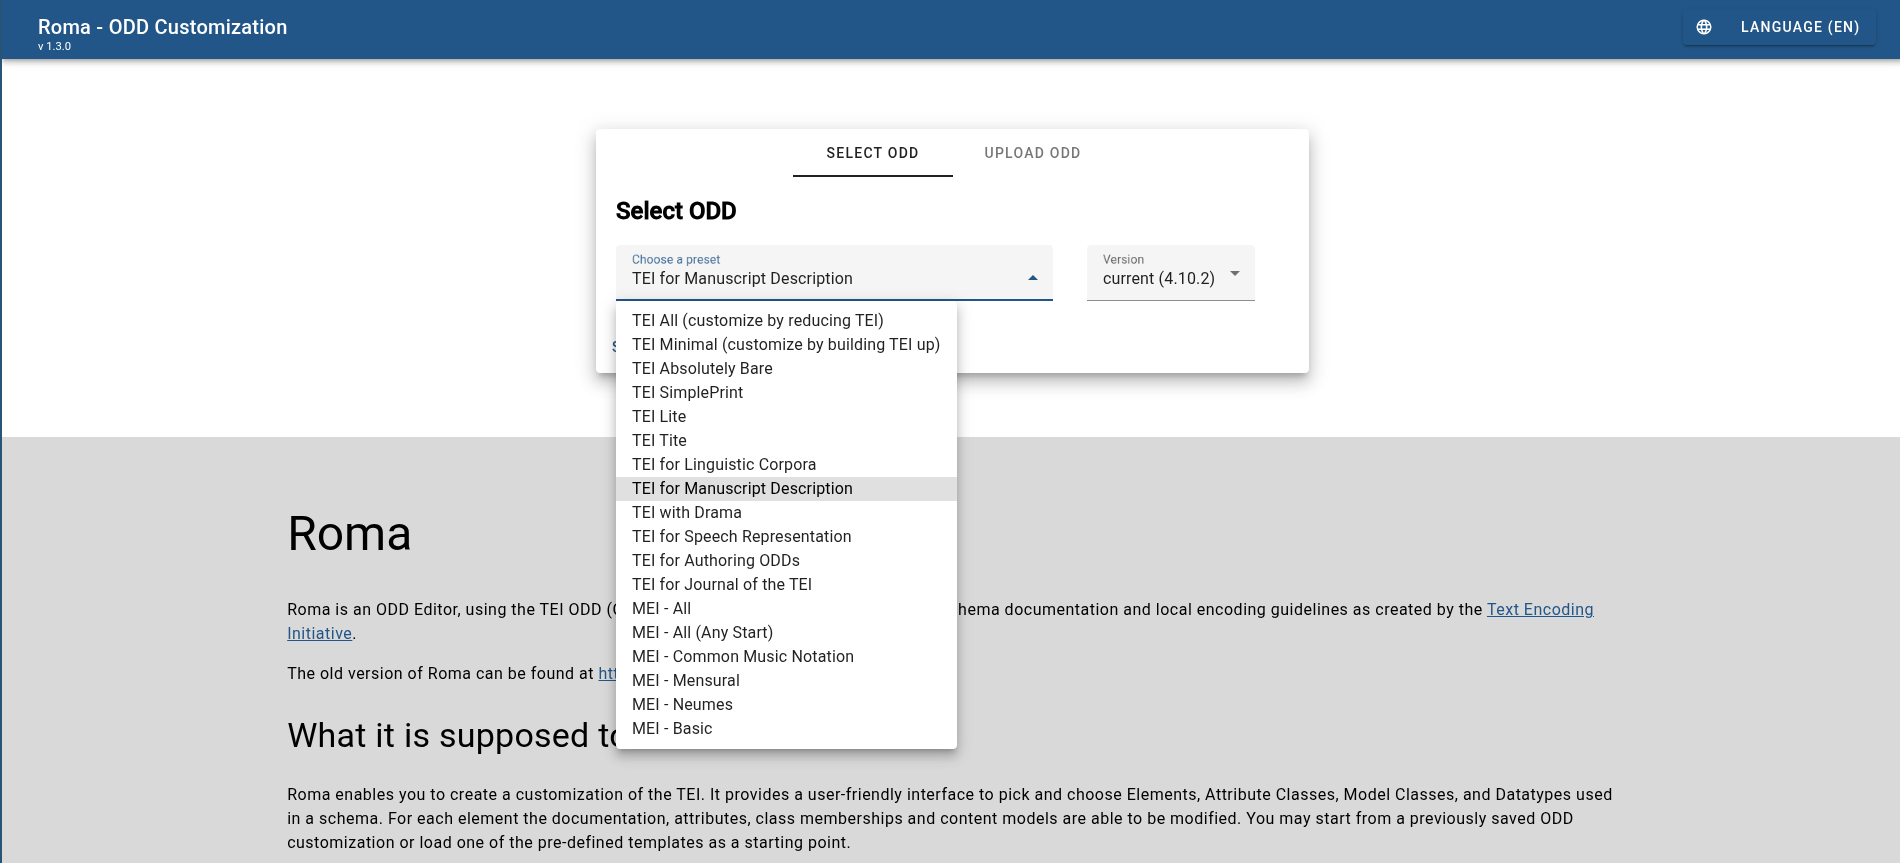
\includegraphics[width=.9\textwidth]{img/roma_main_page.png}
 \caption{La page principale de ROMA: les \enquote{presets}}
\end{figure}
\end{frame}

\begin{frame}{Création de fichiers ODD et de schémas avec ROMA}
\begin{figure}
 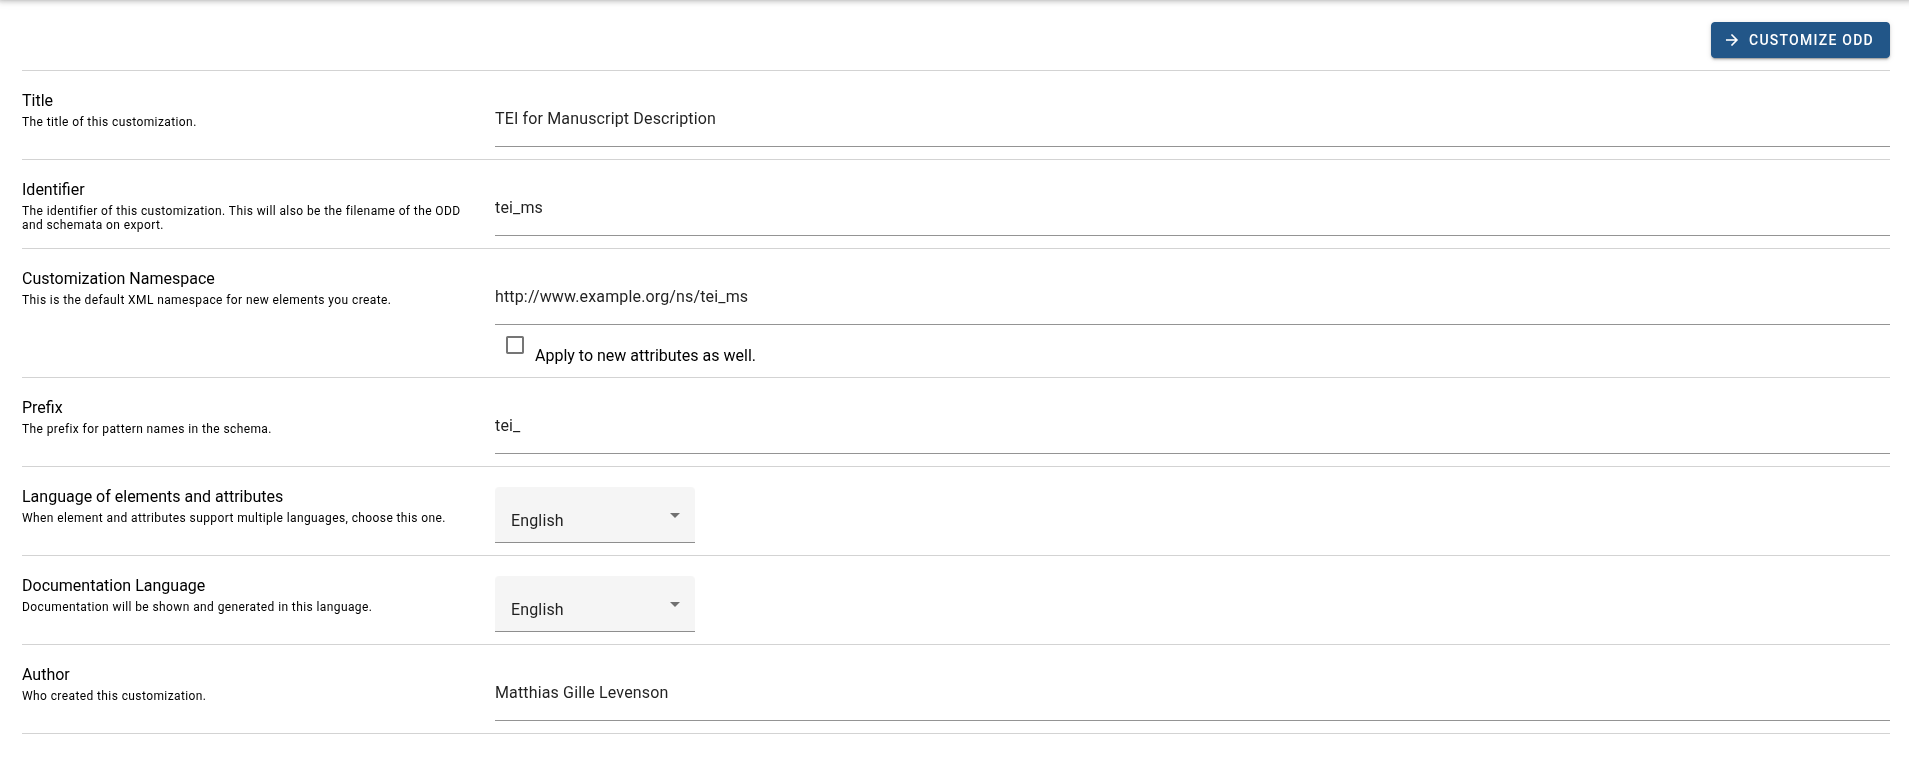
\includegraphics[width=.9\textwidth]{img/settings_odd.png}
 \caption{Configurer l'ODD}
\end{figure}
\end{frame}

\begin{frame}{Création de fichiers ODD et de schémas avec ROMA}
\begin{figure}
 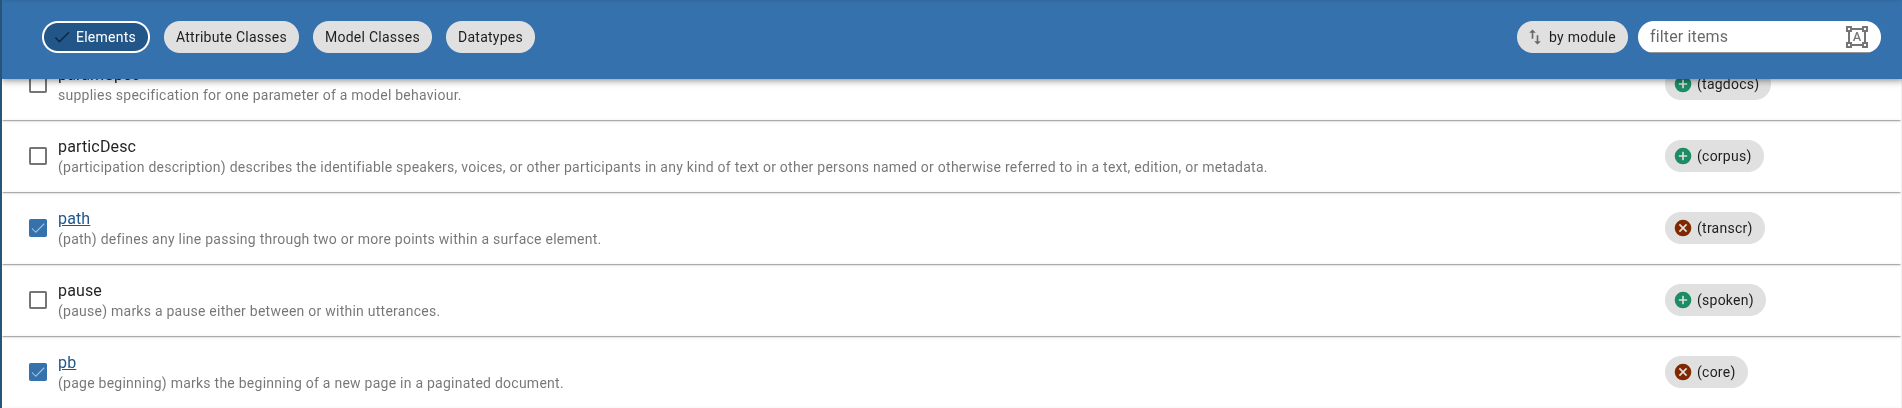
\includegraphics[width=.9\textwidth]{img/finding_pb.png}
 \caption{Recherchez l'élément que vous souhaitez modifier (ici, \texttt{pb})}
\end{figure}
\end{frame}

\begin{frame}{Création de fichiers ODD et de schémas avec ROMA}
\begin{figure}
 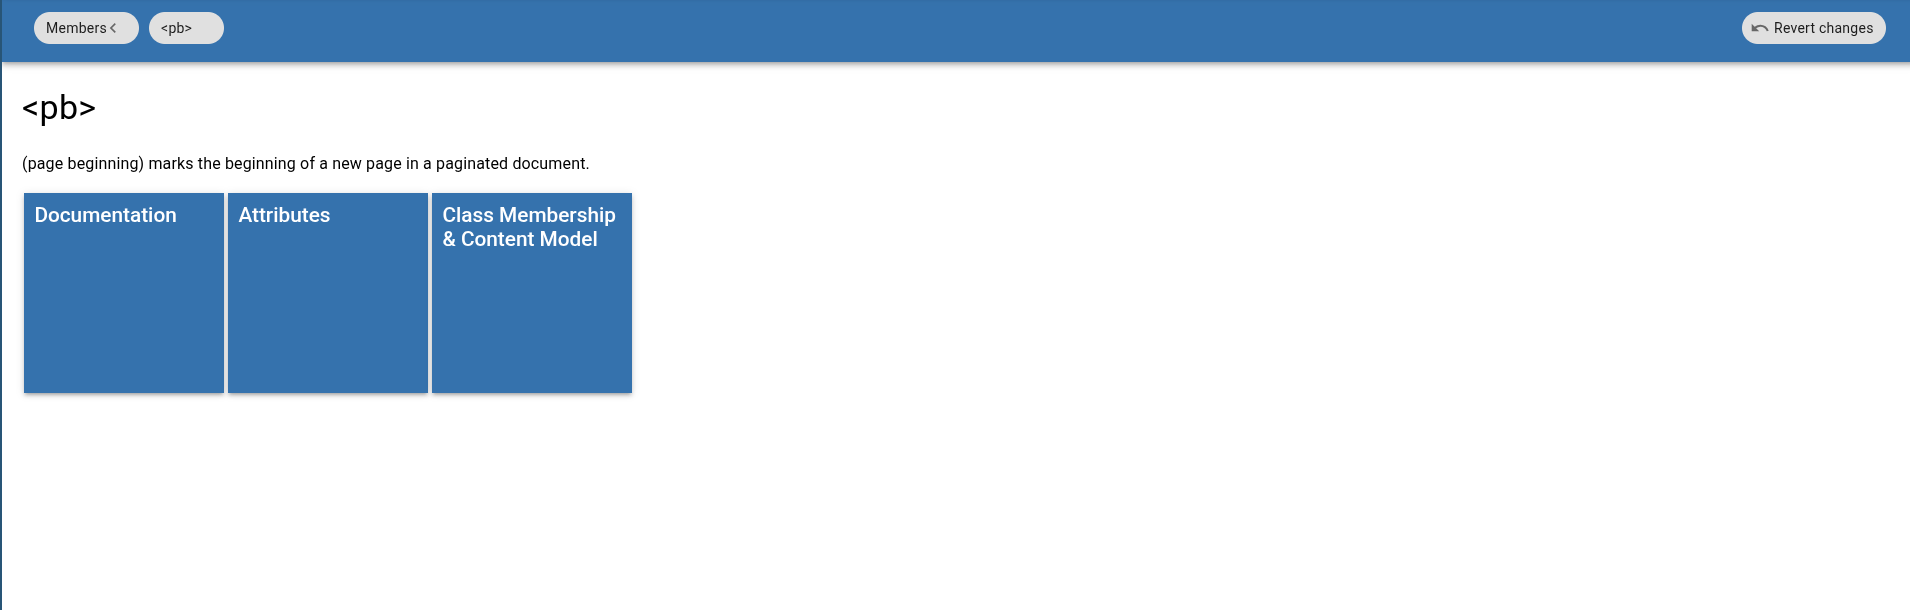
\includegraphics[width=.9\textwidth]{img/feature_selection.png}
 \caption{Choisissez l'élément que vous souhaitez adapter (documentation ou attribut)}
\end{figure}
\end{frame}

\begin{frame}{Création de fichiers ODD et de schémas avec ROMA}
\begin{figure}
 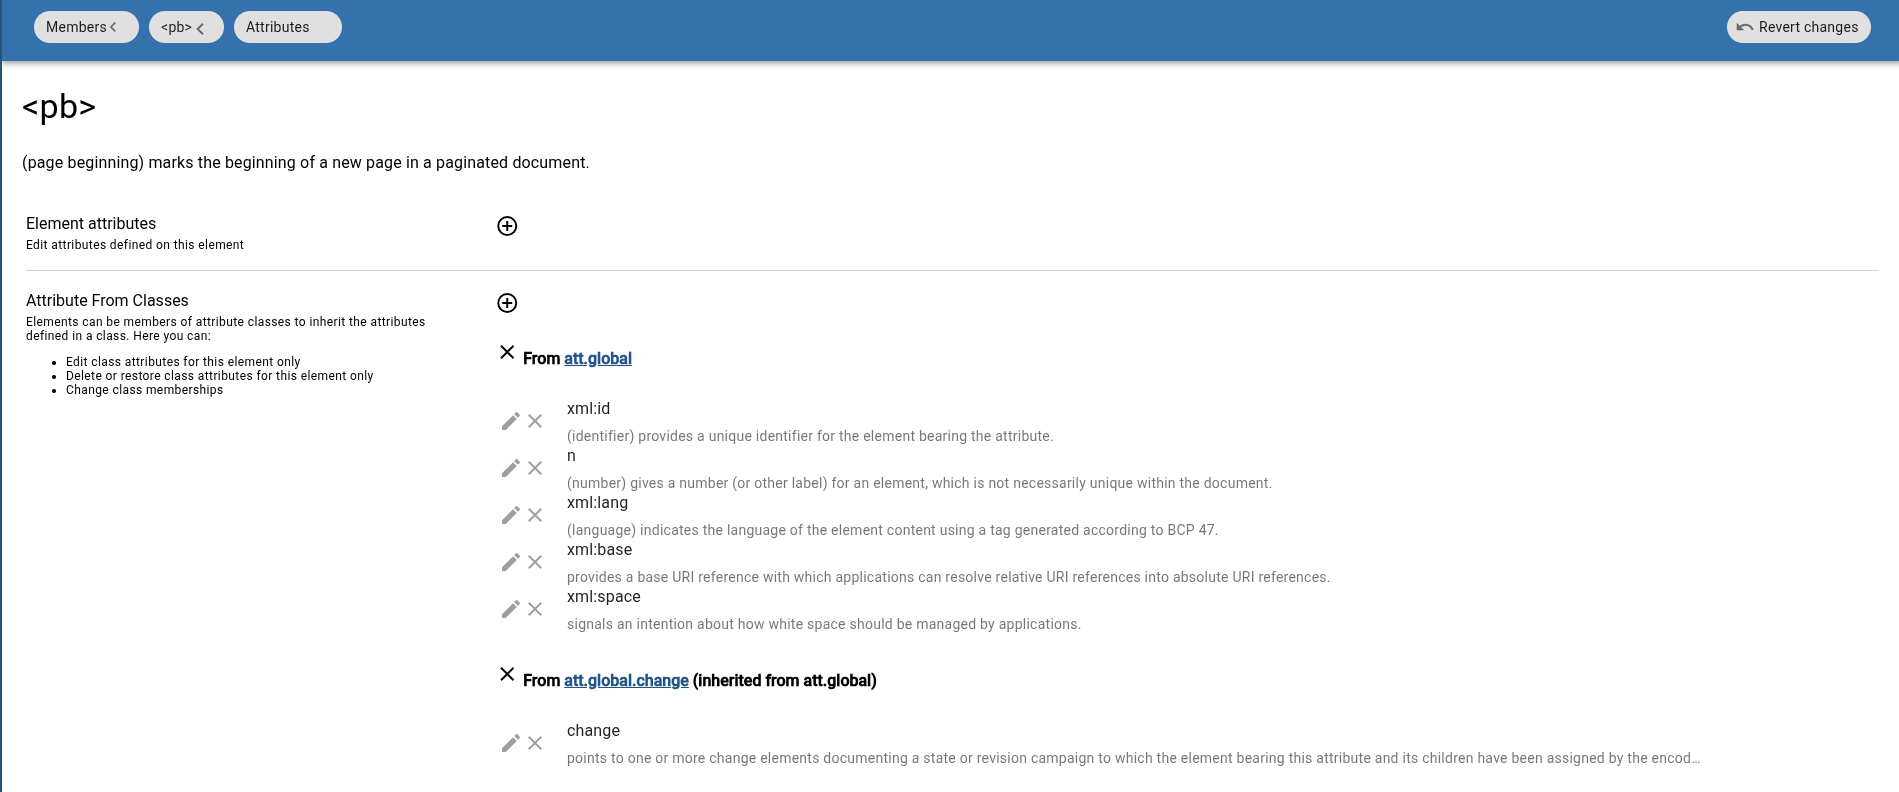
\includegraphics[width=.9\textwidth]{img/attribute_selection.png}
 \caption{Recherchez l'attribut que vous souhaitez modifier}
\end{figure}
\end{frame}

\begin{frame}{Création de fichiers ODD et de schémas avec ROMA}
\begin{figure}
 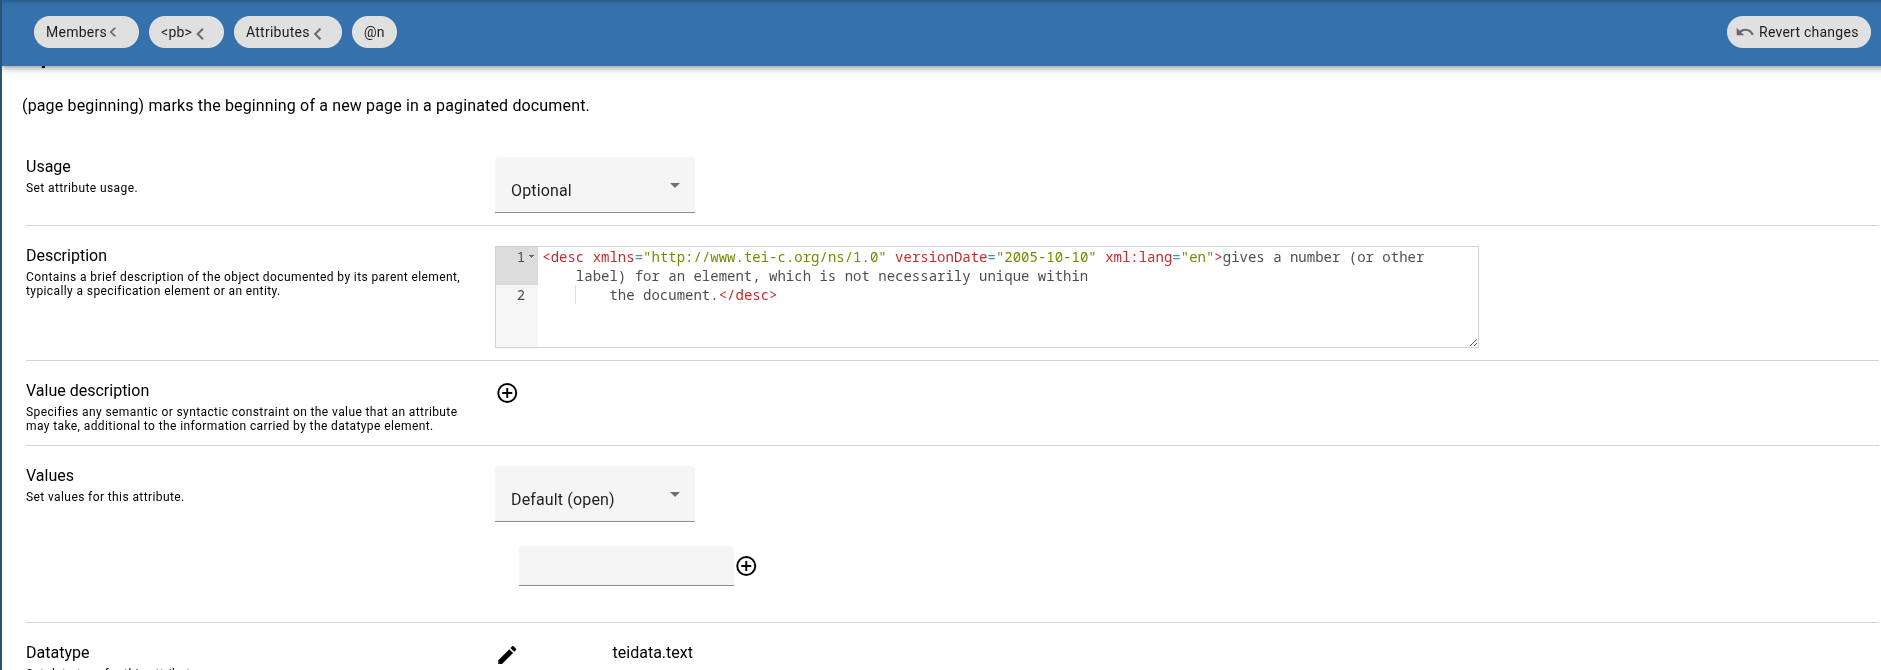
\includegraphics[width=.9\textwidth]{img/changing_attribute_behaviour.png}
 \caption{Changez la façon de l'utiliser ! C'est (presque) automagique !}
\end{figure}
\end{frame}


\begin{frame}{L'ODD produit}
\begin{figure}
 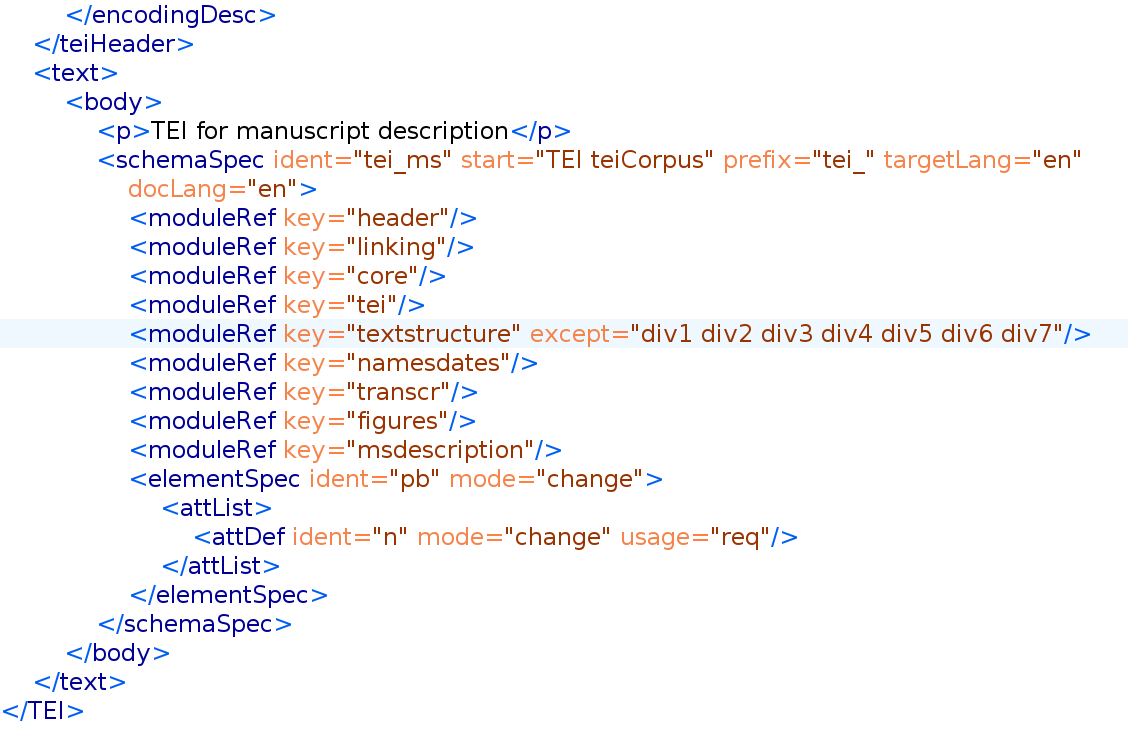
\includegraphics[width=.65\textwidth]{img/my_first_ODD.png}
\end{figure}
Je trouve cette spécification trop générale. Je supprimerais certains modules. Souhaitez-vous décrire des chiffres ? Vous intéressez-vous aux entités nommées ?
\end{frame}



\begin{frame}{Création d'ODD et de schémas avec ROMA : exportation de l'ODD}

% Image vers ROMA
\begin{itemize}
\item Plusieurs formats de sortie. 

\item Le plus important est l'ODD pour les applications scientifiques.

\item Vous aurez besoin de RNC/RNG à des fins de validation. 

\item Vous ne pourrez pas récupérer votre ODD à partir d'un RNG ou de tout autre fichier de schéma.

\item Oxygen peut également générer le schéma à partir des ODD.
\end{itemize}
\end{frame}



\begin{frame}{Faire référence au schéma dans votre fichier TEI}
\begin{figure}
 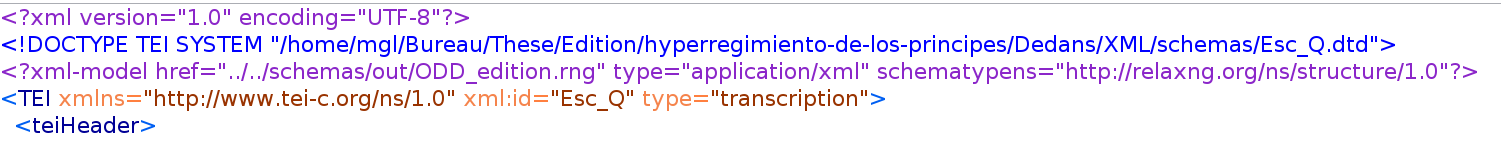
\includegraphics[width=1\textwidth, trim={0 0 0 .2cm}, clip]{img/linking.png}
 \caption{Avant le n\oe ud racine, la référence à mon schéma dérivé de l'ODD (en violet, troisième ligne).}
\end{figure}
\end{frame}




\begin{frame}{Un aperçu de notre ODD}
Résumons. Vous pouvez:
\begin{itemize}
\item Supprimer complètement certains éléments (ils ne seront plus autorisés)

\item Supprimer partiellement certains éléments (ils ne seront autorisés que dans des contextes spécifiques)

\item Restreindre les types d'attributs ou leurs valeurs ; rendre certains attributs obligatoires
\end{itemize}
\end{frame}

%\begin{frame}[fragile]{Activate a module and include selected elements}
%\begin{minted}{xml}
%<moduleRef key="textcrit" include="listWit witness witEnd witStart app rdg"/>
%\end{minted}
%\begin{itemize}
%\item The \texttt{include} attribute means a rebuilding of the module from scratch: absent elements won't be allowed in your encoding
%\item Note here the choice not to include the \texttt{lemma} element, derived from a specific editorial methodology (\enquote{variance}, etc). 
%\end{itemize}
%\end{frame}

%\begin{frame}[fragile]{Make attributes mandatory}
%\begin{minted}{xml}
%<elementSpec ident="pb" mode="change">
%  <attList>
%     <attDef ident="n" mode="change" usage="req"/>
%  </attList>
%</elementSpec>
%\end{minted}
%\end{frame}

%\begin{frame}[fragile]{Remove attributes at element level}
%\begin{minted}{xml}
%<elementSpec ident="material" mode="change" module="msdecription">
%    <attList>
%        <attDef ident="function" mode="delete"/>
%        <attDef ident="target" mode="delete"/>
%        <attDef ident="resp" mode="delete"/>
%        <attDef ident="ref" mode="delete"/>
%    </attList>
%</elementSpec>
%\end{minted}
%\end{frame}

%\begin{frame}[fragile]{Constrain attribute values}
%\begin{minted}[fontsize={\fontsize{9.5}{10.5}\selectfont}]{xml}
%<elementSpec ident="material" mode="change" module="msdecription">
%    <attList>
%        <attDef ident="type" mode="replace" usage="req">
%            <valList mode="add" type="closed">
%                <valItem ident="parchment">
%                    <desc>The copy medium is parchment.</desc>
%                </valItem>
%                <valItem ident="paper">
%                    <desc>The copy medium is paper.</desc>
%                </valItem>
%                <valItem ident="mixt">
%                    <desc>The copy medium alternates between paper and parchment.</desc>
%                </valItem>
%            </valList>
%        </attDef>
%    </attList>
%</elementSpec>
%\end{minted}
%\end{frame}



\begin{frame}{L'autre facette des ODD : la documentation en langage naturel}
% Image vers ROMA
\begin{itemize}
\item Roma n'est que la première étape pour créer la version lisible par machine de votre ODD

\item Comme indiqué précédemment, vous devrez créer et rédiger la documentation \textit{en langage naturel}, en utilisant le TEI. Exemple : \href{https://gitlab.huma-num.fr/mgillelevenson/hyperregimiento-de-los-principes/-/blob/master/Dedans/XML/schemas/ODD_transcriptions.xml?ref_type=heads}{ici}.

\item Vous pouvez utiliser n'importe quel éditeur XML pour ce faire.
\end{itemize}
\begin{figure}
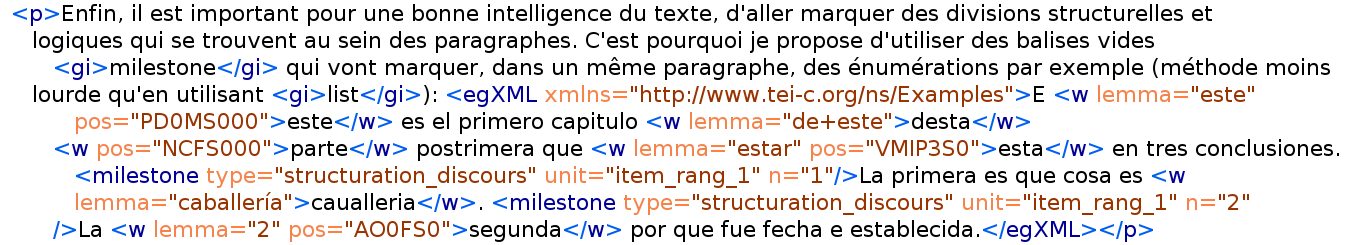
\includegraphics[height=.20\textheight]{img/example_ODD.png}
\caption{Documentation de l'utilisation de \texttt{milestone} dans l'édition du \textit{Regimiento de los prínçipes}.}
\end{figure}
\end{frame}


%\begin{frame}{An example of complete ODD}
%\begin{itemize}
%\item An ODD is an XML-TEI document divided in two parts: the documentation and the schema.
%\item For structuring, use \texttt{div1}...\texttt{div9} elements
%\item You can encode your documentation as you would encode any document
%\item And put you schema specification (the \texttt{schemaSpec}) in a \texttt{div1} for instance.  
%\end{itemize}
%\end{frame}

%\begin{frame}{An example of complete ODD}
%% Image vers ROMA
%\begin{figure}
%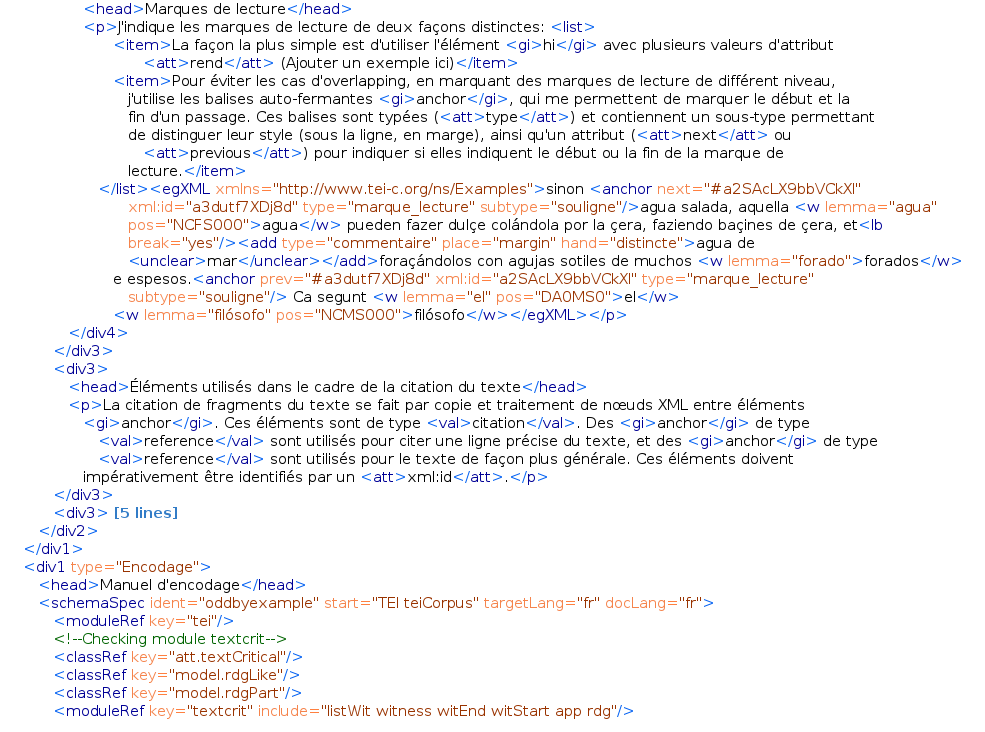
\includegraphics[height=.80\textheight]{img/final_ODD.png}
%\caption{Documenting the use of \texttt{milestone} in the edition of the \textit{Regimiento de los prínçipes}.}
%\end{figure}
%\end{frame}


%\begin{frame}{Respect datatypes plz}
%% Image vers ROMA
%\begin{itemize}
%\item Please make sure you use correctly the elements and attributes described by the TEI consortium
%\item In particular, be aware of datatypes:
%\item For instance, link attributes of class \texttt{teidata.pointer} (\texttt{@ana, @corresp, @sameAs}, etc) are \textit{pointers}, i.e., their datatype is an URI. In general, the URI used in the TEI are relative links, 
%\item When they are not URL, they \textbf{must} start with the hashtag \texttt{\#}.
%\end{itemize}
%\end{frame}



%\begin{frame}[fragile]{Fine-tune the validation with Schematron}
%\begin{minted}{xml}
%<!--The following element can be a child of any elementSpec node-->
%<constraintSpec ident="checks_pb"
%          xmlns:sch="http://purl.oclc.org/dsdl/schematron"
%          xmlns:sqf="http://www.schematron-quickfix.com/validator/process"
%          xmlns:xsl="http://www.w3.org/1999/XSL/Transform"
%          scheme="isoschematron">
%          <constraint>
%            <sch:rule context="tei:pb">
%              <sch:assert test="matches(@n, '\d+[vr]')">Something is wrong with the foliation of
%                this page. Have you forgotten the page side indication
%                ?</sch:assert>
%            </sch:rule>
%          </constraint>
%        </constraintSpec>
%\end{minted}
%\end{frame}


\section{Conclusions}
\begin{frame}{Conclusions}
\begin{itemize}
\item Les Même les schémas les plus simples sont indispensables à tout projet de publication scientifique basé sur TEI.
\item Les éditions basées sur TEI qui ne sont pas accompagnées des sources XML sont pratiquement inutiles et ne feront pas long feu
\item Veuillez donner accès à vos données (et à leur documentation) !
\end{itemize}
\end{frame}


\section{Une dernière chose: ODDbyexample}
\begin{frame}{ODDbyexample}
\begin{itemize}
\item ODDByExample est un outil permettant de générer une spécification ODD à partir d'un document XML-TEI existant

\item Il créera une spécification ODD correspondant à ce document

\item Un outil très utile...

\item ... qui peut toutefois poser problème si l'exemple XML-TEI présente des incohérences : celles-ci seront intégrées à votre spécification

\item Veillez à utiliser cet outil avec des fragments de votre document courts et soigneusement vérifiés.

\item Lien : \href{https://github.com/TEIC/Stylesheets/blob/dev/tools/oddbyexample.xsl}{https://github.com/TEIC/Stylesheets/blob/dev/tools/oddbyexample.xsl}
\end{itemize}
\end{frame}

\section{Exercise}
\begin{frame}{Exercises}
\begin{itemize}
\item Reprenez l'encodage de votre poème, et créez un ODD qui reprend cette modélisation.
\end{itemize}
\end{frame}



\begin{frame}{References}
\printbibliography
\end{frame}

\end{document}
